\section{Sensitivity Analysis}
Sensitivity analysis identifies how the variation of model input
parameters affect select performance 
metrics of the fuel cycle. Additionally, it reveals the combined effect 
of varying multiple parameters on 
an output metric. This information is then used to design 
an optimized transition scenario by identifying which input parameters 
will affect the results the most, and how these parameters should be 
changed to obtain desired results (e.g., minimizing \gls{HALEU} requirements
of a transition). 

\subsection{Methodology}
The analysis was performed on Scenario 7 and Scenario 
14 to provide insight into how the input parameters affect the output 
metrics for both a once-through and recycle fuel cycle. 

\Cyclus was coupled to Dakota \cite{adams_dakota_2019},
and Dakota is the driver for the analysis. This coupling mirrors  
the scripts in the \texttt{dcwrapper} GitHub repository \cite{chee_arfc/dcwrapper_2019}.
Three different types 
of sensitivity analysis were performed: \acrfull{OAT}, synergistic, 
and global. \gls{OAT} analysis varies a single input parameter to 
investigate the effect of each parameter individually. In the context of 
this work, synergistic 
analysis varies two input parameters at once to investigate how the 
interaction of the two parameters affects the results. Finally, the global 
analysis varies more than two input parameters to provide a holistic 
view of how multiple parameters interact and affect the output metrics. 

The input parameters varied include the transition 
start time, the build share of each type of advanced reactor, 
the \gls{LWR} lifetime, and the discharge burnup of fuel from the 
\gls{HALEU}-fueled reactors. The transition start time ranges from January 
2025 to January 2040 in three-month intervals, but the same energy demand 
will be specified for all perturbations (87.20 GWe-yr). The build share 
variable will be repeated three times (for varying the build share of each 
type of advanced reactor) with build share percentages ranging from 0-50\% 
in increments of 5\%. To account for the build share of an advanced reactor
the deployment scheme described in Section \ref{sec:once-through-methods}
was adjusted. Instead of the reactor type with the largest power output 
deployed first, the reactor with the specified build share is deployed first 
until the build share is met. Then the remaining two reactor types are 
deployed in the manner described in Section \ref{sec:once-through-methods},
with the larger of the two reactors preferentially deployed and the smaller 
reactor deployed last to meet the power demand. Figure \ref{fig:build-share-deploy}
illustrates how this deployment scheme is applied to meet a demand of 530 
MWe and a VOYGR build share of 50\%. 

\begin{figure}
    \centering 
    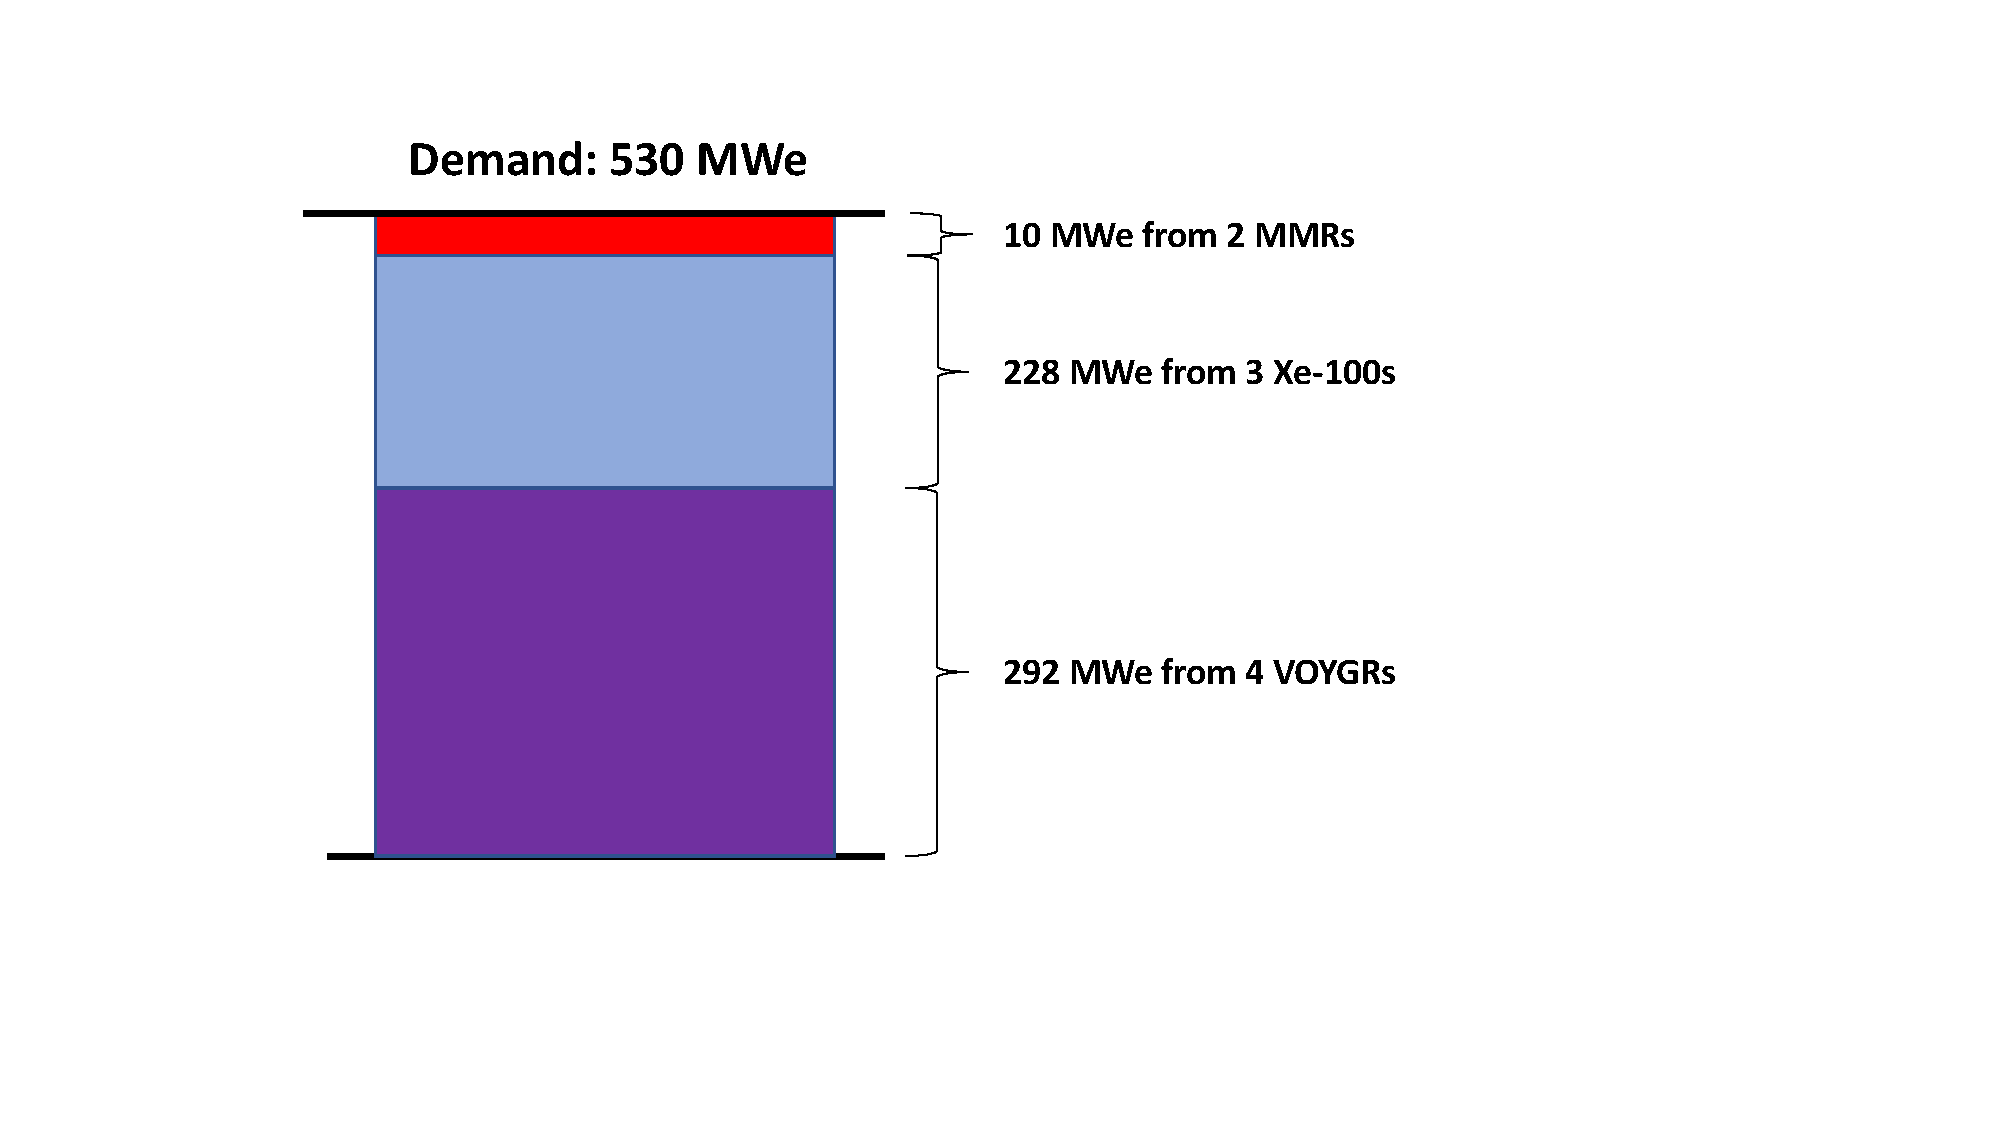
\includegraphics[scale=0.6, trim=50 100 100 0,clip]{VOYGR_build_share.pdf}
    \caption{Demonstration of the adjusted advanced reactor deployment 
    scheme to meet a demand of 530 MWe and a VOYGR build share of 
    50\%.}
    \label{fig:build-share-deploy}
\end{figure}

The \gls{LWR} lifetimes are varied based 
on the percent of the fleet that operate for 60 and 80 years. This 
variable will vary between 0-50\% of the \gls{LWR} fleet operating for 80 
years, while the other \glspl{LWR} operate for 60 years. The 
\glspl{LWR} do not all start operation at the same time, so the 
selection of the \glspl{LWR} that operate for 80 years affects the results, 
even if the number is the same. Therefore, reactors will be selected for 
operation to 80 years in 
descending order of power output, reflecting the greater likelihood of 
larger units receiving a license extension. Previous sensitivity analysis of 
fuel cycle transitions considered the impact of the transition start time 
and the \gls{LWR} lifetimes \cite{chee_sensitivity_2019,feng_sensitivity_2020},
which forms the basis for why these input parameters were selected for this 
work.

\hl{Figure out how to vary the burnup}

The output metrics of 
interest for this analysis include the amount of waste generated that 
must be sent to a repository (\gls{SNF} mass), the mass of enriched uranium, 
the mass of \gls{HALEU},
the amount of \gls{SWU} capacity required to produce all enriched uranium, the 
\gls{SWU} capacity required to produce \gls{HALEU}, and the feed uranium 
required to produce \gls{HALEU}. Each metric will be evaluated based on the 
cumulative sum required, starting at the transition start time. Previous 
sensitivity analysis of fuel cycle transitions considered the waste 
discharged, \gls{SWU} 
capacity required, and natural uranium requirements
\cite{richards_application_2021,feng_sensitivity_2020} 


\subsection{One-at-a-time}

\subsection{Synergistic}

\subsection{Global}

\section{Optimization}